% Options for packages loaded elsewhere
\PassOptionsToPackage{unicode}{hyperref}
\PassOptionsToPackage{hyphens}{url}
\PassOptionsToPackage{dvipsnames,svgnames,x11names}{xcolor}
%
\documentclass[
  letterpaper,
  DIV=11,
  numbers=noendperiod]{scrreprt}

\usepackage{amsmath,amssymb}
\usepackage{iftex}
\ifPDFTeX
  \usepackage[T1]{fontenc}
  \usepackage[utf8]{inputenc}
  \usepackage{textcomp} % provide euro and other symbols
\else % if luatex or xetex
  \usepackage{unicode-math}
  \defaultfontfeatures{Scale=MatchLowercase}
  \defaultfontfeatures[\rmfamily]{Ligatures=TeX,Scale=1}
\fi
\usepackage{lmodern}
\ifPDFTeX\else  
    % xetex/luatex font selection
\fi
% Use upquote if available, for straight quotes in verbatim environments
\IfFileExists{upquote.sty}{\usepackage{upquote}}{}
\IfFileExists{microtype.sty}{% use microtype if available
  \usepackage[]{microtype}
  \UseMicrotypeSet[protrusion]{basicmath} % disable protrusion for tt fonts
}{}
\makeatletter
\@ifundefined{KOMAClassName}{% if non-KOMA class
  \IfFileExists{parskip.sty}{%
    \usepackage{parskip}
  }{% else
    \setlength{\parindent}{0pt}
    \setlength{\parskip}{6pt plus 2pt minus 1pt}}
}{% if KOMA class
  \KOMAoptions{parskip=half}}
\makeatother
\usepackage{xcolor}
\usepackage{svg}
\setlength{\emergencystretch}{3em} % prevent overfull lines
\setcounter{secnumdepth}{5}
% Make \paragraph and \subparagraph free-standing
\ifx\paragraph\undefined\else
  \let\oldparagraph\paragraph
  \renewcommand{\paragraph}[1]{\oldparagraph{#1}\mbox{}}
\fi
\ifx\subparagraph\undefined\else
  \let\oldsubparagraph\subparagraph
  \renewcommand{\subparagraph}[1]{\oldsubparagraph{#1}\mbox{}}
\fi

\usepackage{color}
\usepackage{fancyvrb}
\newcommand{\VerbBar}{|}
\newcommand{\VERB}{\Verb[commandchars=\\\{\}]}
\DefineVerbatimEnvironment{Highlighting}{Verbatim}{commandchars=\\\{\}}
% Add ',fontsize=\small' for more characters per line
\usepackage{framed}
\definecolor{shadecolor}{RGB}{241,243,245}
\newenvironment{Shaded}{\begin{snugshade}}{\end{snugshade}}
\newcommand{\AlertTok}[1]{\textcolor[rgb]{0.68,0.00,0.00}{#1}}
\newcommand{\AnnotationTok}[1]{\textcolor[rgb]{0.37,0.37,0.37}{#1}}
\newcommand{\AttributeTok}[1]{\textcolor[rgb]{0.40,0.45,0.13}{#1}}
\newcommand{\BaseNTok}[1]{\textcolor[rgb]{0.68,0.00,0.00}{#1}}
\newcommand{\BuiltInTok}[1]{\textcolor[rgb]{0.00,0.23,0.31}{#1}}
\newcommand{\CharTok}[1]{\textcolor[rgb]{0.13,0.47,0.30}{#1}}
\newcommand{\CommentTok}[1]{\textcolor[rgb]{0.37,0.37,0.37}{#1}}
\newcommand{\CommentVarTok}[1]{\textcolor[rgb]{0.37,0.37,0.37}{\textit{#1}}}
\newcommand{\ConstantTok}[1]{\textcolor[rgb]{0.56,0.35,0.01}{#1}}
\newcommand{\ControlFlowTok}[1]{\textcolor[rgb]{0.00,0.23,0.31}{#1}}
\newcommand{\DataTypeTok}[1]{\textcolor[rgb]{0.68,0.00,0.00}{#1}}
\newcommand{\DecValTok}[1]{\textcolor[rgb]{0.68,0.00,0.00}{#1}}
\newcommand{\DocumentationTok}[1]{\textcolor[rgb]{0.37,0.37,0.37}{\textit{#1}}}
\newcommand{\ErrorTok}[1]{\textcolor[rgb]{0.68,0.00,0.00}{#1}}
\newcommand{\ExtensionTok}[1]{\textcolor[rgb]{0.00,0.23,0.31}{#1}}
\newcommand{\FloatTok}[1]{\textcolor[rgb]{0.68,0.00,0.00}{#1}}
\newcommand{\FunctionTok}[1]{\textcolor[rgb]{0.28,0.35,0.67}{#1}}
\newcommand{\ImportTok}[1]{\textcolor[rgb]{0.00,0.46,0.62}{#1}}
\newcommand{\InformationTok}[1]{\textcolor[rgb]{0.37,0.37,0.37}{#1}}
\newcommand{\KeywordTok}[1]{\textcolor[rgb]{0.00,0.23,0.31}{#1}}
\newcommand{\NormalTok}[1]{\textcolor[rgb]{0.00,0.23,0.31}{#1}}
\newcommand{\OperatorTok}[1]{\textcolor[rgb]{0.37,0.37,0.37}{#1}}
\newcommand{\OtherTok}[1]{\textcolor[rgb]{0.00,0.23,0.31}{#1}}
\newcommand{\PreprocessorTok}[1]{\textcolor[rgb]{0.68,0.00,0.00}{#1}}
\newcommand{\RegionMarkerTok}[1]{\textcolor[rgb]{0.00,0.23,0.31}{#1}}
\newcommand{\SpecialCharTok}[1]{\textcolor[rgb]{0.37,0.37,0.37}{#1}}
\newcommand{\SpecialStringTok}[1]{\textcolor[rgb]{0.13,0.47,0.30}{#1}}
\newcommand{\StringTok}[1]{\textcolor[rgb]{0.13,0.47,0.30}{#1}}
\newcommand{\VariableTok}[1]{\textcolor[rgb]{0.07,0.07,0.07}{#1}}
\newcommand{\VerbatimStringTok}[1]{\textcolor[rgb]{0.13,0.47,0.30}{#1}}
\newcommand{\WarningTok}[1]{\textcolor[rgb]{0.37,0.37,0.37}{\textit{#1}}}

\providecommand{\tightlist}{%
  \setlength{\itemsep}{0pt}\setlength{\parskip}{0pt}}\usepackage{longtable,booktabs,array}
\usepackage{calc} % for calculating minipage widths
% Correct order of tables after \paragraph or \subparagraph
\usepackage{etoolbox}
\makeatletter
\patchcmd\longtable{\par}{\if@noskipsec\mbox{}\fi\par}{}{}
\makeatother
% Allow footnotes in longtable head/foot
\IfFileExists{footnotehyper.sty}{\usepackage{footnotehyper}}{\usepackage{footnote}}
\makesavenoteenv{longtable}
\usepackage{graphicx}
\makeatletter
\def\maxwidth{\ifdim\Gin@nat@width>\linewidth\linewidth\else\Gin@nat@width\fi}
\def\maxheight{\ifdim\Gin@nat@height>\textheight\textheight\else\Gin@nat@height\fi}
\makeatother
% Scale images if necessary, so that they will not overflow the page
% margins by default, and it is still possible to overwrite the defaults
% using explicit options in \includegraphics[width, height, ...]{}
\setkeys{Gin}{width=\maxwidth,height=\maxheight,keepaspectratio}
% Set default figure placement to htbp
\makeatletter
\def\fps@figure{htbp}
\makeatother
\newlength{\cslhangindent}
\setlength{\cslhangindent}{1.5em}
\newlength{\csllabelwidth}
\setlength{\csllabelwidth}{3em}
\newlength{\cslentryspacingunit} % times entry-spacing
\setlength{\cslentryspacingunit}{\parskip}
\newenvironment{CSLReferences}[2] % #1 hanging-ident, #2 entry spacing
 {% don't indent paragraphs
  \setlength{\parindent}{0pt}
  % turn on hanging indent if param 1 is 1
  \ifodd #1
  \let\oldpar\par
  \def\par{\hangindent=\cslhangindent\oldpar}
  \fi
  % set entry spacing
  \setlength{\parskip}{#2\cslentryspacingunit}
 }%
 {}
\usepackage{calc}
\newcommand{\CSLBlock}[1]{#1\hfill\break}
\newcommand{\CSLLeftMargin}[1]{\parbox[t]{\csllabelwidth}{#1}}
\newcommand{\CSLRightInline}[1]{\parbox[t]{\linewidth - \csllabelwidth}{#1}\break}
\newcommand{\CSLIndent}[1]{\hspace{\cslhangindent}#1}

\KOMAoption{captions}{tableheading}
\makeatletter
\makeatother
\makeatletter
\@ifpackageloaded{bookmark}{}{\usepackage{bookmark}}
\makeatother
\makeatletter
\@ifpackageloaded{caption}{}{\usepackage{caption}}
\AtBeginDocument{%
\ifdefined\contentsname
  \renewcommand*\contentsname{Table of contents}
\else
  \newcommand\contentsname{Table of contents}
\fi
\ifdefined\listfigurename
  \renewcommand*\listfigurename{List of Figures}
\else
  \newcommand\listfigurename{List of Figures}
\fi
\ifdefined\listtablename
  \renewcommand*\listtablename{List of Tables}
\else
  \newcommand\listtablename{List of Tables}
\fi
\ifdefined\figurename
  \renewcommand*\figurename{Figure}
\else
  \newcommand\figurename{Figure}
\fi
\ifdefined\tablename
  \renewcommand*\tablename{Table}
\else
  \newcommand\tablename{Table}
\fi
}
\@ifpackageloaded{float}{}{\usepackage{float}}
\floatstyle{ruled}
\@ifundefined{c@chapter}{\newfloat{codelisting}{h}{lop}}{\newfloat{codelisting}{h}{lop}[chapter]}
\floatname{codelisting}{Listing}
\newcommand*\listoflistings{\listof{codelisting}{List of Listings}}
\makeatother
\makeatletter
\@ifpackageloaded{caption}{}{\usepackage{caption}}
\@ifpackageloaded{subcaption}{}{\usepackage{subcaption}}
\makeatother
\makeatletter
\@ifpackageloaded{tcolorbox}{}{\usepackage[skins,breakable]{tcolorbox}}
\makeatother
\makeatletter
\@ifundefined{shadecolor}{\definecolor{shadecolor}{rgb}{.97, .97, .97}}
\makeatother
\makeatletter
\makeatother
\makeatletter
\makeatother
\ifLuaTeX
  \usepackage{selnolig}  % disable illegal ligatures
\fi
\IfFileExists{bookmark.sty}{\usepackage{bookmark}}{\usepackage{hyperref}}
\IfFileExists{xurl.sty}{\usepackage{xurl}}{} % add URL line breaks if available
\urlstyle{same} % disable monospaced font for URLs
\hypersetup{
  pdftitle={IM939\_handbook\_quarto},
  pdfauthor={Norah Jones},
  colorlinks=true,
  linkcolor={blue},
  filecolor={Maroon},
  citecolor={Blue},
  urlcolor={Blue},
  pdfcreator={LaTeX via pandoc}}

\title{IM939\_handbook\_quarto}
\author{Norah Jones}
\date{2023-08-14}

\begin{document}
\maketitle
\ifdefined\Shaded\renewenvironment{Shaded}{\begin{tcolorbox}[sharp corners, borderline west={3pt}{0pt}{shadecolor}, interior hidden, enhanced, breakable, frame hidden, boxrule=0pt]}{\end{tcolorbox}}\fi

\renewcommand*\contentsname{Table of contents}
{
\hypersetup{linkcolor=}
\setcounter{tocdepth}{2}
\tableofcontents
}
\bookmarksetup{startatroot}

\hypertarget{preface}{%
\chapter*{Preface}\label{preface}}
\addcontentsline{toc}{chapter}{Preface}

\markboth{Preface}{Preface}

This is a Quarto book.

To learn more about Quarto books visit
\url{https://quarto.org/docs/books}.

\begin{Shaded}
\begin{Highlighting}[]
\DecValTok{1} \OperatorTok{+} \DecValTok{1}
\end{Highlighting}
\end{Shaded}

\begin{verbatim}
2
\end{verbatim}

\bookmarksetup{startatroot}

\hypertarget{introduction}{%
\chapter{Introduction}\label{introduction}}

This is a book created from markdown and executable code.

See Knuth (1984) for additional discussion of literate programming.

\begin{Shaded}
\begin{Highlighting}[]
\DecValTok{1} \OperatorTok{+} \DecValTok{1}
\end{Highlighting}
\end{Shaded}

\begin{verbatim}
2
\end{verbatim}

\bookmarksetup{startatroot}

\hypertarget{im939---lab-1---part-1}{%
\chapter{IM939 - Lab 1 - Part 1}\label{im939---lab-1---part-1}}

Welcome to the first Python lab.

Our aim is to introduce a little bit of Python and help you be
comfortable with using Jupyter notebooks. No previous knowledge is
assumed and questions are encouraged!

Please make sure you have Anaconda Python installed and running on your
computer. Instructions for doing this on a Windows 10 machine can be
found in the video below. There is a little code before the video which
is needed to display the video in the notebook, you can ignore this for
now.

For your convenience, the installation files for anaconda for each
platform are linked below.

\href{https://repo.anaconda.com/archive/Anaconda3-2020.07-Windows-x86_64.exe}{Windows}
\href{https://repo.anaconda.com/archive/Anaconda3-2020.07-MacOSX-x86_64.pkg}{MacOS}

\hypertarget{python}{%
\section{Python?}\label{python}}

Python is a very popular general purpose programming language. Data
scientists use it to clean up, analyse and visualise data. A major
strength of python is that the core Python functionality can be extended
using libraries. In future labs, you will learn about popular data
science libraries such as pandas and numpy.

It is useful to think of programming languages as a structured way to
tell the computer what to do. We cover some of the basic features of
Python in this lab.

\hypertarget{anaconda}{%
\subsection{Anaconda}\label{anaconda}}

\href{https://anaconda.org/}{Anaconda} is a collection of different
programs. These programs include Python, many of the most popular data
science libaries, Jupyter notebooks and development environments such as
\href{https://code.visualstudio.com/}{VS Code} or
\href{https://www.spyder-ide.org/}{Spyder}, which are Integrated
Development Environments (IDEs) that we can use for python.

\hypertarget{jupter-notebooks}{%
\subsection{Jupter Notebooks}\label{jupter-notebooks}}

Jupyter notebooks, such as this one, allow you to combine text and code
into documents you can edit in the browser. The power of these notebooks
is in documenting or describing what you are doing with the code
alongside that code. For example, you could detail why you chose a
particular clustering algorithm above the clustering code itself. In
other words, it add narrative and helps clarify your workflow.

\hypertarget{getting-started}{%
\section{Getting started}\label{getting-started}}

If you send Python a number then it will print that number for you.

\begin{Shaded}
\begin{Highlighting}[]
\DecValTok{45}
\end{Highlighting}
\end{Shaded}

\begin{verbatim}
45
\end{verbatim}

You will see both the input and output displayed. The input will have a
label next to it like `In {[}1{]}' where the number tells you how much
code has already been sent to the Python interpreter (the programming
interpreting the Python code and returnign the result). A line such as
`In {[}100{]}' tells you that 99 code cells have been passed to the
Python interpreter in the current session.

Python can carry out simple arithetic.

\begin{Shaded}
\begin{Highlighting}[]
\DecValTok{44} \OperatorTok{+} \DecValTok{87}
\end{Highlighting}
\end{Shaded}

\begin{verbatim}
131
\end{verbatim}

\begin{Shaded}
\begin{Highlighting}[]
\DecValTok{188} \OperatorTok{/} \DecValTok{12}
\end{Highlighting}
\end{Shaded}

\begin{verbatim}
15.666666666666666
\end{verbatim}

\begin{Shaded}
\begin{Highlighting}[]
\DecValTok{46} \OperatorTok{{-}} \DecValTok{128}
\end{Highlighting}
\end{Shaded}

\begin{verbatim}
-82
\end{verbatim}

Each time the code in the cell is run and the result from the Python
interpreter is displayed.

\bookmarksetup{startatroot}

\hypertarget{data-types}{%
\chapter{Data Types}\label{data-types}}

\hypertarget{int-floats-strings}{%
\section{int, floats, strings}\label{int-floats-strings}}

Integers are whole numbers. We used them above.

You can also have floats (numbers with decimal points)

\begin{Shaded}
\begin{Highlighting}[]
\FloatTok{33.4}
\end{Highlighting}
\end{Shaded}

\begin{verbatim}
33.4
\end{verbatim}

and a series of characters (strings).

\begin{Shaded}
\begin{Highlighting}[]
\CommentTok{\textquotesingle{}I have a plan, sir.\textquotesingle{}}
\end{Highlighting}
\end{Shaded}

\begin{verbatim}
'I have a plan, sir.'
\end{verbatim}

Data types are great and operators such as * do different things
depending on the data type. For instance,

\begin{Shaded}
\begin{Highlighting}[]
\DecValTok{33} \OperatorTok{*} \DecValTok{3}
\end{Highlighting}
\end{Shaded}

\begin{verbatim}
99
\end{verbatim}

That seems quite sensible. What about if we had a string? Run teh below
line. What is the * doing?

\begin{Shaded}
\begin{Highlighting}[]
\CommentTok{\textquotesingle{}I have a plan, sir\textquotesingle{}} \OperatorTok{*} \DecValTok{3}
\end{Highlighting}
\end{Shaded}

\begin{verbatim}
'I have a plan, sirI have a plan, sirI have a plan, sir'
\end{verbatim}

There are also operators which only work with particular data types.

\begin{Shaded}
\begin{Highlighting}[]
\CommentTok{\# \textquotesingle{}I have a plan, sir.\textquotesingle{} / 2}
\end{Highlighting}
\end{Shaded}

This error message is very informative indeed. It tells us the line
which caused the problem and that we have an error. Specifically, our
error is a TypeError.

The line

`I have a cunning plan' / 2

consists of

string / int

We are trying to divide a string and int. The / operand is not able to
divide a string by an int.

\hypertarget{lists-and-dictionaries}{%
\subsection{lists and dictionaries}\label{lists-and-dictionaries}}

You can collect multiple values in a list.

\begin{Shaded}
\begin{Highlighting}[]
\NormalTok{[}\DecValTok{35}\NormalTok{, }\StringTok{\textquotesingle{}brown\textquotesingle{}}\NormalTok{, }\StringTok{\textquotesingle{}yes\textquotesingle{}}\NormalTok{]}
\end{Highlighting}
\end{Shaded}

\begin{verbatim}
[35, 'brown', 'yes']
\end{verbatim}

Or add keys to the values as a dictionary.

\begin{Shaded}
\begin{Highlighting}[]
\NormalTok{\{}\StringTok{\textquotesingle{}age\textquotesingle{}}\NormalTok{:}\DecValTok{35}\NormalTok{, }\StringTok{\textquotesingle{}hair colour\textquotesingle{}}\NormalTok{: }\StringTok{\textquotesingle{}brown\textquotesingle{}}\NormalTok{, }\StringTok{\textquotesingle{}Glasses\textquotesingle{}}\NormalTok{: }\StringTok{\textquotesingle{}yes\textquotesingle{}}\NormalTok{\}}
\end{Highlighting}
\end{Shaded}

\begin{verbatim}
{'age': 35, 'hair colour': 'brown', 'Glasses': 'yes'}
\end{verbatim}

\bookmarksetup{startatroot}

\hypertarget{variables}{%
\chapter{Variables}\label{variables}}

Variables are bins for storing things in. These things can be data
types. For example, the below creates a variable called my\_height and
stores the in 140 there.

\begin{Shaded}
\begin{Highlighting}[]
\NormalTok{my\_height }\OperatorTok{=} \DecValTok{140}
\end{Highlighting}
\end{Shaded}

The Python interpreter is now storing the int 140 in a bin called
my\_height. If you pass the variable name to the interpreter then it
will behave just like if you typed in 140 instead.

\begin{Shaded}
\begin{Highlighting}[]
\NormalTok{my\_height}
\end{Highlighting}
\end{Shaded}

\begin{verbatim}
140
\end{verbatim}

140

Variables are neat when it comes to lists.

\begin{Shaded}
\begin{Highlighting}[]
\NormalTok{my\_heights }\OperatorTok{=}\NormalTok{ [}\DecValTok{231}\NormalTok{, }\DecValTok{234}\NormalTok{, }\DecValTok{43}\NormalTok{]}
\NormalTok{my\_heights}
\end{Highlighting}
\end{Shaded}

\begin{verbatim}
[231, 234, 43]
\end{verbatim}

\begin{Shaded}
\begin{Highlighting}[]
\NormalTok{my\_heights[}\DecValTok{1}\NormalTok{]}
\end{Highlighting}
\end{Shaded}

\begin{verbatim}
234
\end{verbatim}

Wait, what happened above? What do you think the {[}1{]} does?

You can index multiple values from a list.

\begin{Shaded}
\begin{Highlighting}[]
\NormalTok{my\_heights[}\DecValTok{0}\NormalTok{:}\DecValTok{2}\NormalTok{]}
\end{Highlighting}
\end{Shaded}

\begin{verbatim}
[231, 234]
\end{verbatim}

\hypertarget{bringing-it-all-together}{%
\section{Bringing it all together}\label{bringing-it-all-together}}

What does the below do?

\begin{Shaded}
\begin{Highlighting}[]
\NormalTok{radius }\OperatorTok{=} \DecValTok{40}
\NormalTok{pi }\OperatorTok{=} \FloatTok{3.1415}
\NormalTok{circle\_area }\OperatorTok{=}\NormalTok{ pi }\OperatorTok{*}\NormalTok{ (radius }\OperatorTok{*}\NormalTok{ radius)}

\NormalTok{length }\OperatorTok{=} \DecValTok{12}
\NormalTok{square\_area }\OperatorTok{=}\NormalTok{ length }\OperatorTok{*}\NormalTok{ length}

\NormalTok{my\_areas }\OperatorTok{=}\NormalTok{ [circle\_area, square\_area]}
\end{Highlighting}
\end{Shaded}

\begin{Shaded}
\begin{Highlighting}[]
\NormalTok{my\_areas}
\end{Highlighting}
\end{Shaded}

\begin{verbatim}
[5026.400000000001, 144]
\end{verbatim}

As an aside, you can include comments which are not evaluated by the
Python interpreter.

\begin{Shaded}
\begin{Highlighting}[]
\CommentTok{\# this is a number}
\CommentTok{\# another comment}
\NormalTok{n }\OperatorTok{=} \DecValTok{33}
\end{Highlighting}
\end{Shaded}

\bookmarksetup{startatroot}

\hypertarget{congratulations}{%
\chapter{Congratulations}\label{congratulations}}

You've reached the end of the first notebook. We've looked at basic data
type and variables. These are key components of all programming
languages and a key part of working with data.

In the next notebook we will examine using libraries, loading in data,
loops and functions.

\bookmarksetup{startatroot}

\hypertarget{content-with-notebooks}{%
\chapter{Content with notebooks}\label{content-with-notebooks}}

You can also create content with Jupyter Notebooks. This means that you
can include code blocks and their outputs in your book.

\hypertarget{markdown-notebooks}{%
\section{Markdown + notebooks}\label{markdown-notebooks}}

As it is markdown, you can embed images, HTML, etc into your posts!

\includesvg{https://myst-parser.readthedocs.io/en/latest/_static/logo-wide.svg}

You can also \(add_{math}\) and

\[
math^{blocks}
\]

or

\[
\begin{aligned}
\mbox{mean} la_{tex} \\ \\
math blocks
\end{aligned}
\]

But make sure you \$Escape \$your \$dollar signs \$you want to keep!

\hypertarget{myst-markdown}{%
\section{MyST markdown}\label{myst-markdown}}

MyST markdown works in Jupyter Notebooks as well. For more information
about MyST markdown, check out
\href{https://jupyterbook.org/content/myst.html}{the MyST guide in
Jupyter Book}, or see
\href{https://myst-parser.readthedocs.io/en/latest/}{the MyST markdown
documentation}.

\hypertarget{code-blocks-and-outputs}{%
\section{Code blocks and outputs}\label{code-blocks-and-outputs}}

Jupyter Book will also embed your code blocks and output in your book.
For example, here's some sample Matplotlib code:

\begin{Shaded}
\begin{Highlighting}[]
\ImportTok{from}\NormalTok{ matplotlib }\ImportTok{import}\NormalTok{ rcParams, cycler}
\ImportTok{import}\NormalTok{ matplotlib.pyplot }\ImportTok{as}\NormalTok{ plt}
\ImportTok{import}\NormalTok{ numpy }\ImportTok{as}\NormalTok{ np}
\NormalTok{plt.ion()}
\end{Highlighting}
\end{Shaded}

\begin{verbatim}
<matplotlib.pyplot._IonContext at 0x10566c640>
\end{verbatim}

\begin{Shaded}
\begin{Highlighting}[]
\CommentTok{\# Fixing random state for reproducibility}
\NormalTok{np.random.seed(}\DecValTok{19680801}\NormalTok{)}

\NormalTok{N }\OperatorTok{=} \DecValTok{10}
\NormalTok{data }\OperatorTok{=}\NormalTok{ [np.logspace(}\DecValTok{0}\NormalTok{, }\DecValTok{1}\NormalTok{, }\DecValTok{100}\NormalTok{) }\OperatorTok{+}\NormalTok{ np.random.randn(}\DecValTok{100}\NormalTok{) }\OperatorTok{+}\NormalTok{ ii }\ControlFlowTok{for}\NormalTok{ ii }\KeywordTok{in} \BuiltInTok{range}\NormalTok{(N)]}
\NormalTok{data }\OperatorTok{=}\NormalTok{ np.array(data).T}
\NormalTok{cmap }\OperatorTok{=}\NormalTok{ plt.cm.coolwarm}
\NormalTok{rcParams[}\StringTok{\textquotesingle{}axes.prop\_cycle\textquotesingle{}}\NormalTok{] }\OperatorTok{=}\NormalTok{ cycler(color}\OperatorTok{=}\NormalTok{cmap(np.linspace(}\DecValTok{0}\NormalTok{, }\DecValTok{1}\NormalTok{, N)))}


\ImportTok{from}\NormalTok{ matplotlib.lines }\ImportTok{import}\NormalTok{ Line2D}
\NormalTok{custom\_lines }\OperatorTok{=}\NormalTok{ [Line2D([}\DecValTok{0}\NormalTok{], [}\DecValTok{0}\NormalTok{], color}\OperatorTok{=}\NormalTok{cmap(}\FloatTok{0.}\NormalTok{), lw}\OperatorTok{=}\DecValTok{4}\NormalTok{),}
\NormalTok{                Line2D([}\DecValTok{0}\NormalTok{], [}\DecValTok{0}\NormalTok{], color}\OperatorTok{=}\NormalTok{cmap(}\FloatTok{.5}\NormalTok{), lw}\OperatorTok{=}\DecValTok{4}\NormalTok{),}
\NormalTok{                Line2D([}\DecValTok{0}\NormalTok{], [}\DecValTok{0}\NormalTok{], color}\OperatorTok{=}\NormalTok{cmap(}\FloatTok{1.}\NormalTok{), lw}\OperatorTok{=}\DecValTok{4}\NormalTok{)]}

\NormalTok{fig, ax }\OperatorTok{=}\NormalTok{ plt.subplots(figsize}\OperatorTok{=}\NormalTok{(}\DecValTok{10}\NormalTok{, }\DecValTok{5}\NormalTok{))}
\NormalTok{lines }\OperatorTok{=}\NormalTok{ ax.plot(data)}
\NormalTok{ax.legend(custom\_lines, [}\StringTok{\textquotesingle{}Cold\textquotesingle{}}\NormalTok{, }\StringTok{\textquotesingle{}Medium\textquotesingle{}}\NormalTok{, }\StringTok{\textquotesingle{}Hot\textquotesingle{}}\NormalTok{])}\OperatorTok{;}
\end{Highlighting}
\end{Shaded}

\begin{figure}[H]

{\centering 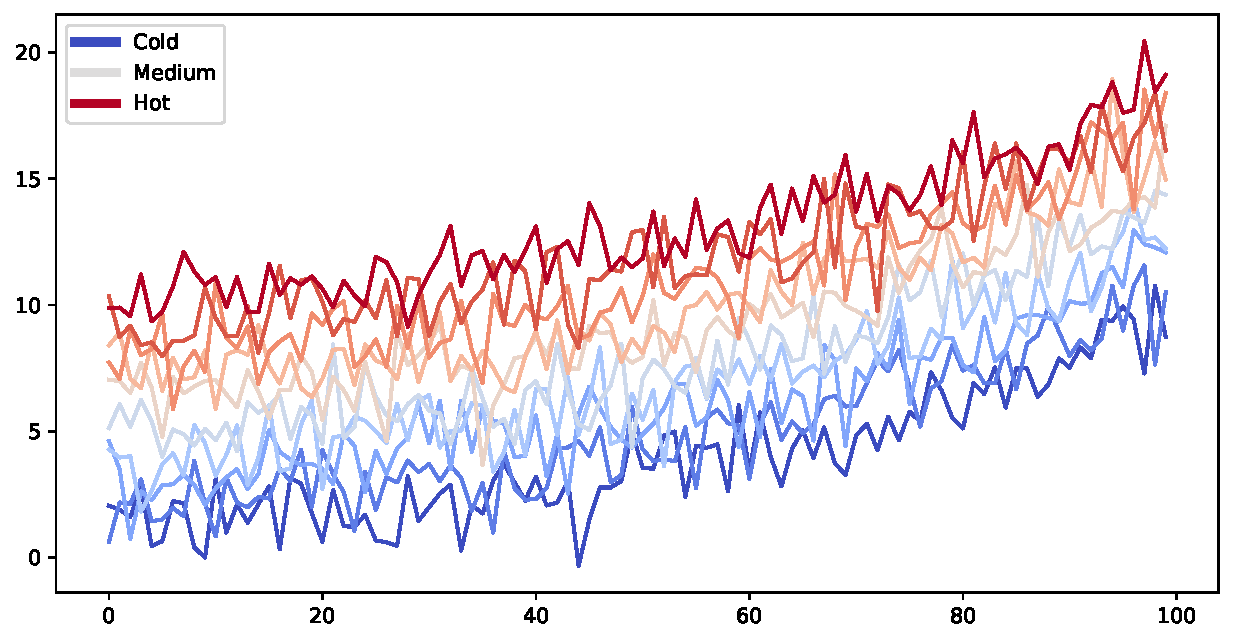
\includegraphics{content/jupyterbook-demo/notebooks_files/figure-pdf/cell-3-output-1.pdf}

}

\end{figure}

There is a lot more that you can do with outputs (such as including
interactive outputs) with your book. For more information about this,
see \href{https://jupyterbook.org}{the Jupyter Book documentation}

\bookmarksetup{startatroot}

\hypertarget{summary}{%
\chapter{Summary}\label{summary}}

In summary, this book has no content whatsoever.

\begin{Shaded}
\begin{Highlighting}[]
\DecValTok{1} \OperatorTok{+} \DecValTok{1}
\end{Highlighting}
\end{Shaded}

\begin{verbatim}
2
\end{verbatim}

\bookmarksetup{startatroot}

\hypertarget{references}{%
\chapter*{References}\label{references}}
\addcontentsline{toc}{chapter}{References}

\markboth{References}{References}

\hypertarget{refs}{}
\begin{CSLReferences}{1}{0}
\leavevmode\vadjust pre{\hypertarget{ref-knuth84}{}}%
Knuth, Donald E. 1984. {``Literate Programming.''} \emph{Comput. J.} 27
(2): 97--111. \url{https://doi.org/10.1093/comjnl/27.2.97}.

\end{CSLReferences}



\end{document}
